\section{DETERMINISTIC SCORES}
\subsection{Spearman rank correlation}

Spearman's correlation is a non-parametric measure of rank correlation 
(statistical dependence between the rankings of two variables). 
It assesses how well the relationship between two variables can be described using a monotonic function (whether linear or not).  

$$r_s=\frac{cov(R[H],R[O])}{\sigma_{R[H]} \cdot \sigma_{R[O]}}$$
where : \\

\begin{itemize}
	\item $r_s : $ spearman rand correlation 
	\item H : the Hindcast.
	\item O : the Observation.
	\item R[x] : the rank of the variable x. 
	\item $\sigma_x : $ standard deviation of the variable x.
\end{itemize}

The analysis of The rank correlation in our case show that the DWD() model is the best in the MENA region in all lead times.

\begin{figure}[H]
	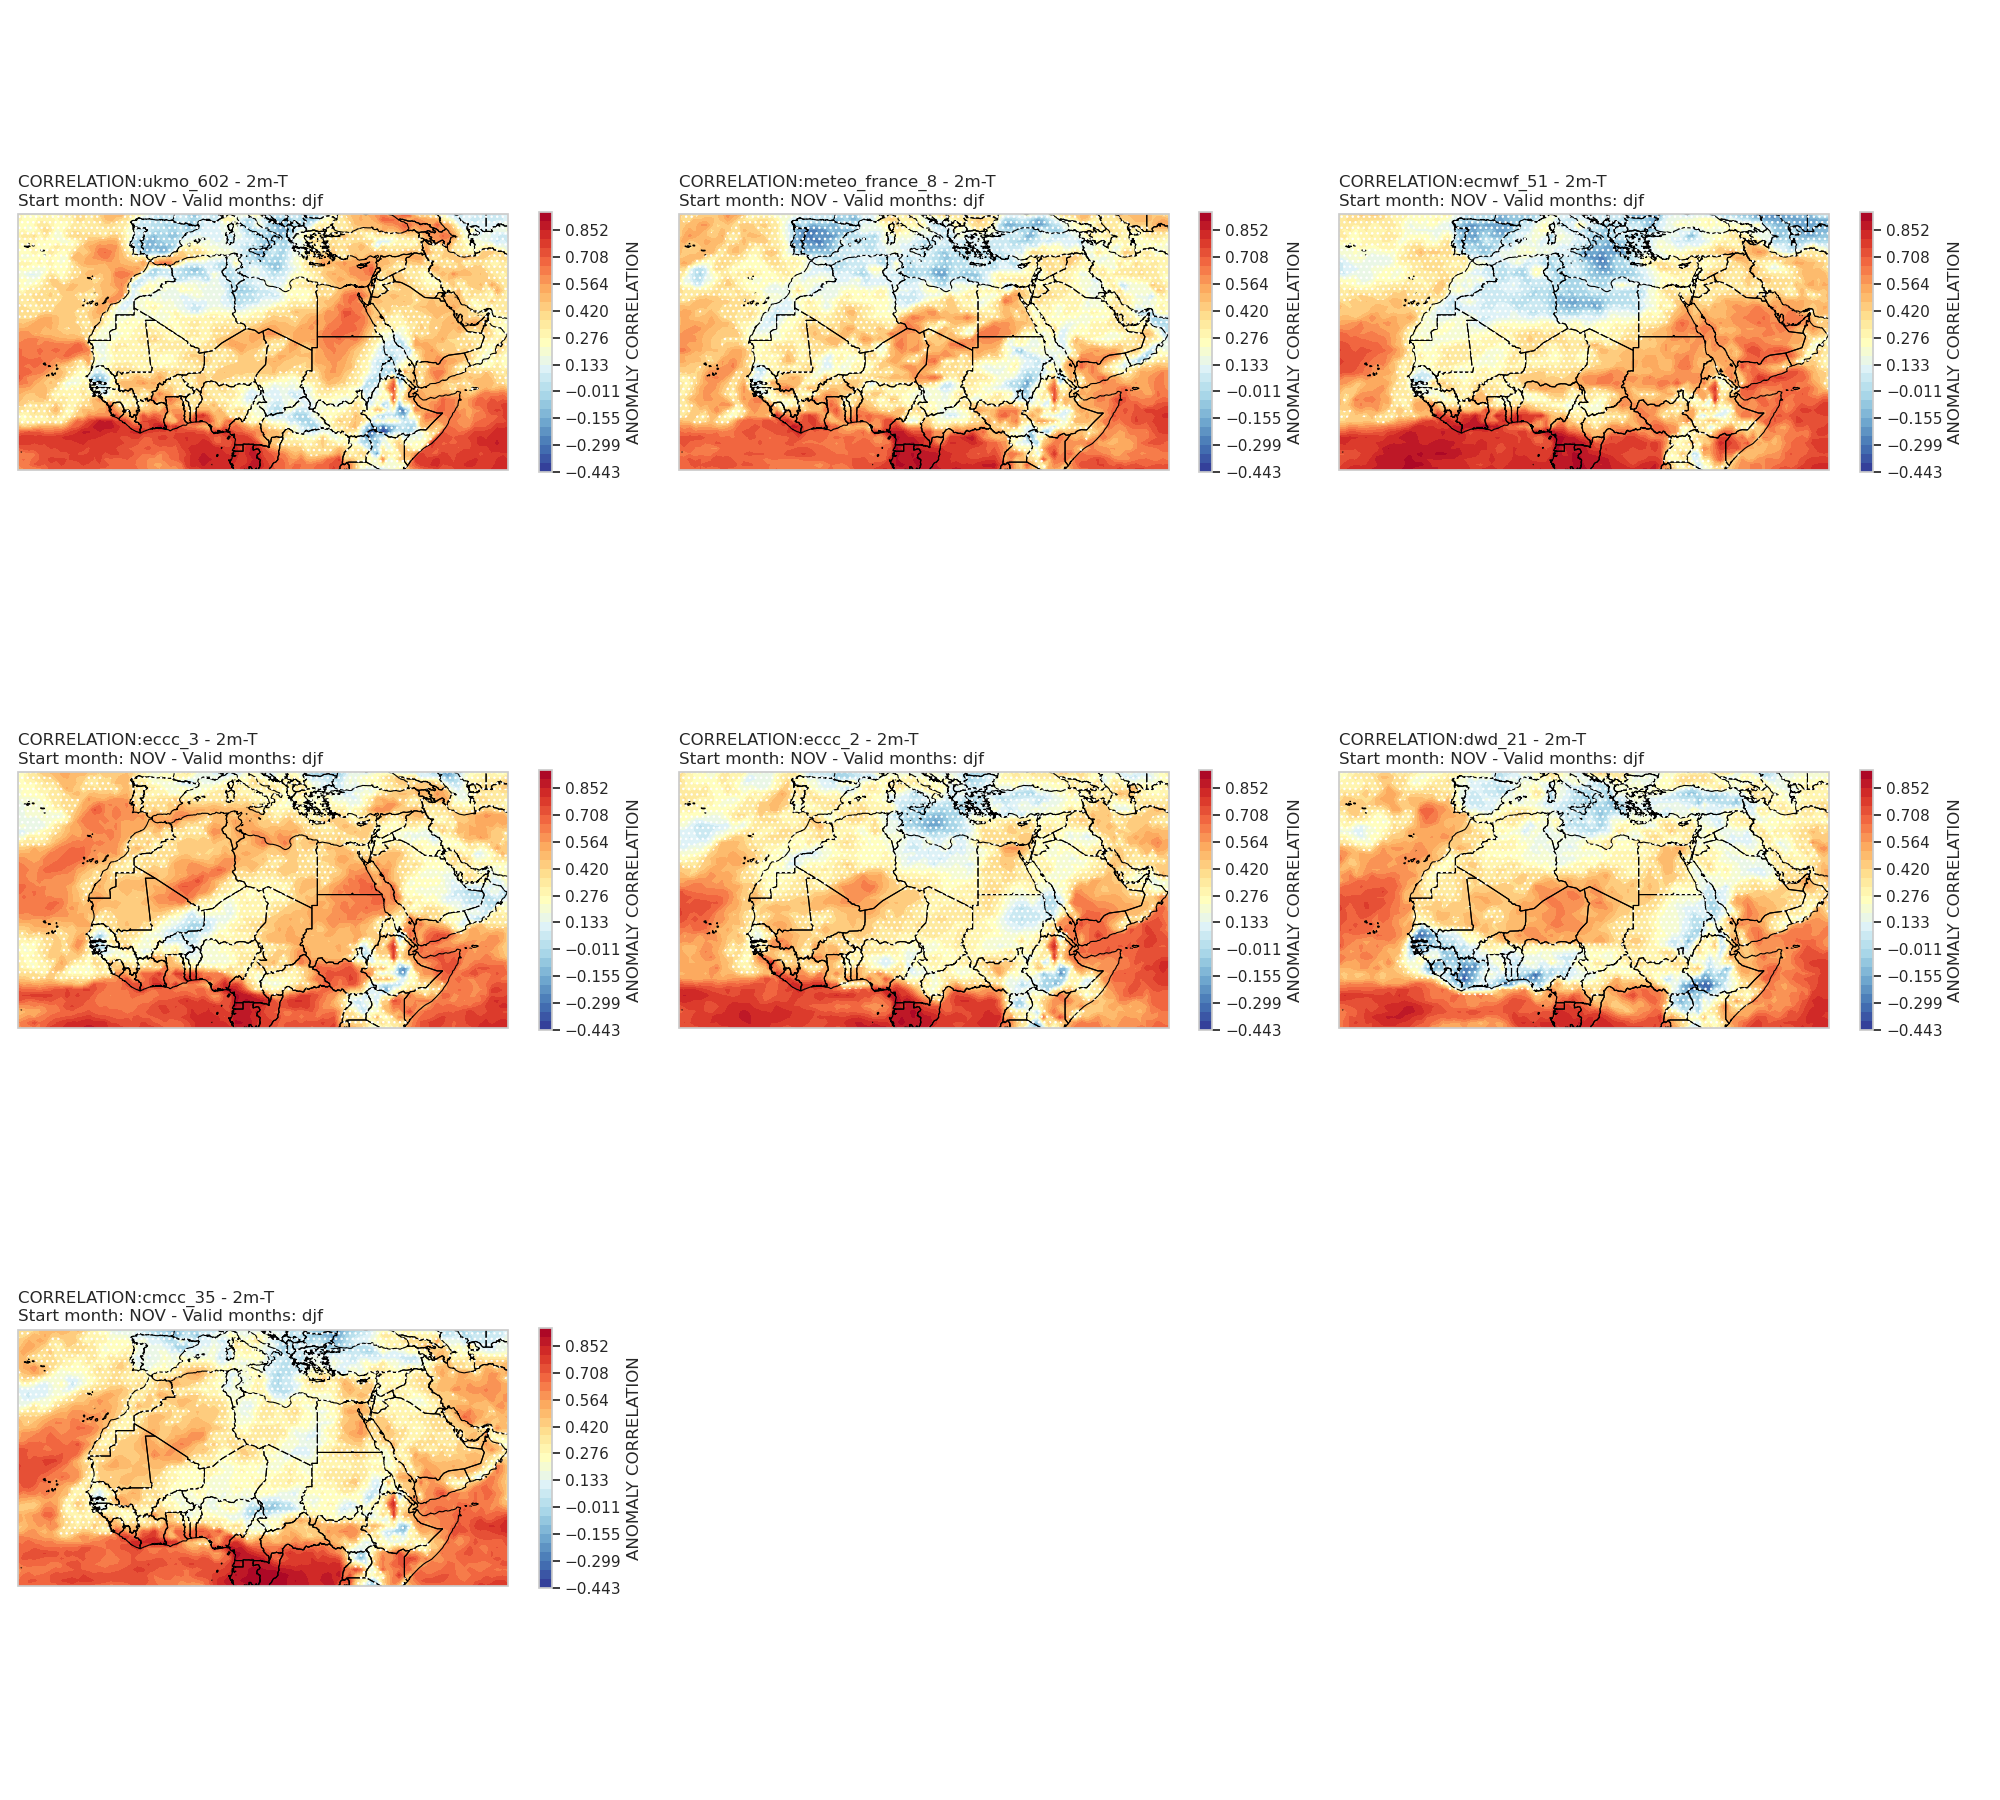
\includegraphics[scale=0.2]{CORR_DJF.png}
	\caption{Spearman Correlation on different centers 3-month rolling mean DJF }
\end{figure}

 \subsection{RMSE}
 
 $RMSE$ measures the average difference between a the hindcast and the observation.
 
$$RMSE=\sqrt{\frac{1}{n} \sum\limits_{i=1}^{n}(H_i -O_i)^2}$$
where :
\begin{itemize}
	\item H : the Hindcast.
	\item O : the observation.
	\item i : the valid time.
\end{itemize}